\documentclass[11pt]{beamer}
\usepackage[UTF8]{ctex}
\usepackage[utf8]{inputenc}
\usepackage[T1]{fontenc}
\usepackage{lmodern}
\usepackage{amsmath}
\usepackage{amsfonts}
\usepackage{amssymb}
\usepackage{graphicx}
\usetheme{CambridgeUS}

\usepackage{pdfpages}


%%%%%
\usepackage{longtable}
\usepackage{subfigure}
\usepackage{color}
\usepackage{booktabs}

%%%%%
\usepackage[backend=bibtex,sorting=none]{biblatex}
\addbibresource{reference.bib} %BibTeX数据文件及位置
\setbeamerfont{footnote}{size=\tiny} 
\setbeamertemplate{bibliography item}[text]

%% LOGO放右上
\setbeamertemplate{frametitle}
{\begin{beamercolorbox}[wd=\paperwidth]{frametitle}
		\strut\hspace{0.5em}\insertframetitle\strut
		\hfill
		\raisebox{-2mm}{
\includegraphics[width=1cm]{figures/HNUC.jpeg}}
	\end{beamercolorbox}
}

%%% 绘图
\usepackage{pgfplots}
\pgfplotsset{width=7cm,compat=1.13}
\usepackage{pgf-pie} % 饼图

%%% 课件属性定义
\author{郭泰彪}
\title{区块链原理及应用}
\subtitle{第10课:区块链在实体经济中的应用}
\institute[湖工商大数据研究院]{湖南工商大学大数据与互联网创新研究院}
\date{2020年11月12日}
\titlegraphic{
\includegraphics[width=2cm]{figures/HNUC.jpeg}}

\begin{document}
\begin{frame}
	\maketitle
\end{frame}

\begin{frame}
	\frametitle{目录}
	\tableofcontents[sectionstyle=show,subsectionstyle=show/shaded]
\end{frame}

\section{区块链助力知识产权步入新纪元}

\begin{frame}
	\frametitle{}
	{\Large 	区块链助力知识产权步入新纪元}
\end{frame}


\begin{frame}{知识产权行业概况}
	知识产权,也称其为“知识所属权”,指“权利人对其智力劳动所创作的成果和经营活动中的标记、信誉所依法享有的专有权利”。知识产权是关于人类在社会实践中创造的智力劳动成果的专有权利。随着科技的发展,为了更好保护产权人的利益,知识产权制度应运而生并不断完善。

	知识产权行业从横向市场来看分为版权市场、专利市场、商标市场;从纵向环节分为确权、用权和维权,其中确权主要指版权申请、登记、复议和认证等业务,用权主要涉及版权授权、收费和交易等业务,维权主要是侵权调查、预警和诉讼等服务,与法律制定等息息相关。
\end{frame}


\begin{frame}
	\frametitle{2014-2018年专利、商标申请量与增长率\footnote{数据来源:国家知识产权局}}
	\begin{minipage}[t]{0.5\linewidth}
		\begin{figure}
			\begin{tikzpicture}[scale=0.8]
				\tiny
				\begin{axis}[
						ybar,
						enlargelimits=0.15,
						legend style={at={(0.5,-0.15)},
								anchor=north,legend columns=-1},
						symbolic x coords={2014,2015,2016,2017,2018},
						xtick=data,
						nodes near coords,
						nodes near coords align={vertical},
					]
					\addplot coordinates {(2014,231) (2015,278) (2016,342) (2017,363) (2018,432)};
					\addplot coordinates {(2014,228) (2015,285) (2016,350) (2017,574) (2018,737)};
					\legend{专利申请量:万件(发明、实用新型、外观专利),商标申请数量:万件}
				\end{axis}
			\end{tikzpicture}
		\end{figure}
	\end{minipage}%
	% 此行用于空格
	\begin{minipage}[t]{0.05\linewidth}
		\quad
	\end{minipage}%
	\begin{minipage}[t]{0.4\linewidth}
		\begin{figure}
			。2018年我国专利申请量(包括发明专利、实用新型和外观设计)为432.3万件,同比增长16.9\%,近五年来专利申请总量增长近一倍;2018年我国商标注册申请量达到737.1万件,同比增长28.2\%,近五年来商标注册申请量增长约2.5倍;在著作权方面,作品、计算机软件著作权登记量分别达235万件、110万件,同比分别增长17.48\%、48.22\%
		\end{figure}
	\end{minipage}
\end{frame}

\subsection{知识产权行业的四大痛点}

\begin{frame}{知识产权行业的四大痛点}
	\begin{enumerate}
		\item 确权流程繁琐且耗时,降低权利人积极性
		      % 知识产权的确权作为知识产权后续用权、维权的第一步,流程复杂且繁琐,甚至有些知识产权的确权需要支付一定的费用,一定程度上降低了权利人确权的积极性。以专利确权为例,专利法要求申请人提交专门的专利申请文件,在专利说明书中充分公开技术方案,然后撰写权利要求以明确保护范围。不仅如此,专利局还要对专利权利要求进行实质审查,只有在确认它符合专利法规定的授权要件之后,才授予专利权。另外,权利人还要缴纳各种费用以支付政府进行事先审查的成本。因为确权流程复杂方繁琐,耗时长,所以催生出一些知识产权代理人,代理当事人处理知识产权事务。以版权代理确权为例,对比国内三家知名的互联网版权代理,发现整个流程至少需要1周时间左右,甚至最长接近2个月时间;另外费用最低也在598元/件起步,有一定门槛。
		\item 知识产权估值困难,商业化程度低
		      % 由于知识产权属于无形资产,确定知识产权的评估标准是世界性难题。无形资产多,创新性产权多,这对评估标准的细化造成了一定的困难;并且从从业人员角度看,评估师需要懂法律、会计,又要懂得知识产权和金融,也对从业人员提出了一定的要求。根据国家知识产权局的调研显示,我国知识产权质押融资存在着规模小、成本高、融资难、周期长等问题。2018年全国著作权登记总量达到345.7万件,相比2017年的274.8万件,同比增长25.83%,显示出我国在知识产权供给方面的能力已有大幅提升。如果将目前的知识产权质押规模与我国巨大的知识产权存量相比,可以发现知识产权质押融资比例并不高,我国知识产权质押融资规模与中国的新增贷款和社会融资规模相比也比较低。例如,2018年,我国新增贷款达到16.17万亿,社会融资规模总量为19.26万亿元,专利、商标及版权质押融资1224亿元,只占新增信贷额的0.76%,占社会融资额0.64%。另外,由于对知识产权评估价值认可度不高,导致知识产权抵押融资的授信额度较低,与知识产权的评估价值差距较大。如某银行发明专利权的授信额不超过评估值的25%,实用新型专利权的授信额不超过评估值的15%,商标专用权的授信额不超过评估值的30%。总体来看我国知识产权估值困难,供给充足,但整体商业化程度低。
		\item 产权溯源难,维权效率低下
		      % 维权是知识产权中较为重要的环节之一,产权溯源难,维权效率低下是目前知识产权服务业在维权环节面临的问题之一。另外随着数字时代的发展,侵权界定和权力溯源也变得更为困难。以音像版权为例,首先侵权界定需要逐级查阅授权说明,其次,音像产品因为权力分割情况严重,往往有多个主体对单一音像产品拥有权力主张,比如词曲人拥有著作权,歌手拥有版权,音像发行公司拥有发行权,以及其他主体拥有复制权、播放权等等,这些权力分割和权力交叉现象,导致对权力溯源和侵权界定形成巨大困难。另外,由于我国法律属于“谁主张谁举证”性质,被侵权人往往需要自己收集证据举证侵权行为,包括调查侵权行为人所侵权的程度,包括使用情况、销售数量等,以此测算产权人遭受的经济损失,并且这些证据还需要满足法庭对证据严谨性的要求。而后需要提起诉讼,而诉讼将会花费非常大的时间和精力,流程繁荣复杂,效率低下。
		\item 知产变现分配机制不透明、不合理
		      % 知产收益分配不透明、不合理,也是当前知产变现环节面临的问题之一。知识产权属于无形资产,其拥有的价值属性更多的是产权人的创造所带来的,但在现在的知产市场上,有非常多的知产变现分配机制不合理的现象,包括音乐版权领域、书籍版权领域等等,变现的价值更多的被渠道所攥取,真正的创造者却没有获得应有的价值分配。比如在音乐版权行业中,据MIDiA研究报告数据显示,每张专辑流向歌手的价值仅占全部变现价值的14.3%,流向作曲者的收益仅为9.5%,大部分的价值被发行平台所攥取。
	\end{enumerate}
\end{frame}

\subsection{区块链如何为知识产权行业赋能}

\begin{frame}{区块链如何为知识产权行业赋能}
	\begin{enumerate}
		\item 区块链提升确权效率,降低确权成本
		      % 传统知识产权的确权流程繁荣复杂,耗时长,是由于整体的确权流程大部分由人工完成。比如在著作权确权过程中,需要递交必须的文件资料进行审查,且著作权实行登记制,其确权仅仅是形式审查,并非实质审查,即相关机构仅对递交的材料是否符合相应的申请要求进行审查,并且不违反《著作权法》的规定即可获权,而不对著作权的内容进行审查。形式审查是整个知识产权确权中最简单的流程,但目前的著作权确权仍需要至少一个月左右的时间。顺应国家对知识产权发展的要求,已经出现了一些线上确权登记的互联网企业,能够在线上实现对版权的快速确权登记。但各互联网企业各自为政,企业各自之间不开放相应数据,且司法对这类线上版权的证据能力、证据效力认可度不同,造成这类互联网确权企业对知识产权的确权和用权、维权环节出现断层。而区块链的去中介化和可信时间戳的不可篡改性,能够推动知识产权行业发展,实现巨大跨越。利用区块链和可信时间戳对知识产权进行存证,能够对每个知识产权生成独一无二且不可篡改的存在性证明;另外,知识产权区块链通过连接司法机关,让司法机关成为知识产权区块链节点,能够为链上存证提供强大公信力,修复后续用权、维权与确权的断层。
		\item 智能合约助力链上知识产权流转,提升知产变现效率
		      % 首先,知识产权通过确权环节已经实现数字化和上链,通过区块链上的信息可以快速明确产权主体。清晰的产权主体能够为知识产权的变现提供助力。需求人可以通过链上信息快速找到产权主体,实现供需双方的快速连接。结合大数据和人工智能技术,对知识产权实现高效的、精准的供需匹配,一定程度提升知识产权的变现率。
		      % 其次,产权人可以通过智能合约实现对产权的良好管理,提升产权变现效率。产权人可以通过为知识产权设定对应的智能合约,将产权人的诉求写入智能合约,并通过私钥进行签名。只要需求人满足产权人写在智能合约中的诉求,那么智能合约就可以自动为需求人授权,并在授权期限到期时将授权停止,甚至可以实现对同个知识产权匹配不同的诉求和开放权限。通过智能合约管理知识产权,能够很大程度上解放产权人和需求人,消除传统知产变现中的代理人环节,自动化管理自动化管理知识产权的流转和变现,极大提升知识产权的流转效率。
		\item 助力产权溯源,明确权力界定,提升维权效率
		      % 由于知识产权的确权行为在链上完成,链上保存有知识产权的完整信息,配合无法篡改的时间戳,能够真实反映知识产权的历史存在证明。并且通过链上信息,能够明确追溯知识产权的拥有人,也能够快速确定知识产权的权力界定。另外,产权人可以通过调用知识产权区块链上的侵权取证固证功能,对相应的侵权行为进行固证,将侵权行为写入区块链,并同时明确侵权主体,借用区块链的无法篡改的特性,使侵权行为一旦发生就无法抵赖。链上固证相比传统人工收集证据,能够极大压缩证据收集的时间,降低举证成本,简化流程并提高效率。另外,知识产权区块链通过连接产权中心、司法机关等政府机构,能够为链上数据提供强有力的公信力,并且整合了产权中心、司法机关等政府机构的知识产权区块链,其上存储的固证能够满足司法机关对证据的要求,司法机关能够依据链上证据对侵权案件进行快速审判,极大简化法院审判流程,提升维权效率。并且最终通过调动产权人的维权动力,降低侵权行为的发生。
		\item 智能合约助力产权变现,提高价值分配合理性
		      % 在知识产权上链前,可以明确各权利人的权益分配、权限资格等,当权利各方达成一致意见,将其写入区块链上的智能合约,以实现共识的、透明的价值分配。当链上发生知识产权的变现授权时,通过智能合约即可自动将收入分配给相关权益人,实现变现权益的透明分配。另外,由于传统知识产权变现一部分会通过代理人执行,代理人也会分走一部分的知识产权变现权益。而通过智能合约管理知识产权,并依托强大的大数据和人工智能技术,能够实现精确匹配知识产权需求者,消除产权变现中代理人环节,将原本被代理人剥夺的价值进行重新分配,提高价值分配合理性。
	\end{enumerate}
\end{frame}

\subsection{区块链+知识产权落地项目仍面临一定的困难点}

\begin{frame}{区块链+知识产权落地项目仍面临一定的困难点}
	% 现有国内落地区块链+知识产权保护平台,基本上是采用联盟链形式,利用区块链技术拥有的不可篡改、可追溯、可信时间戳的特性,对知识产权拥有人的作品进行上链存证,并通过后台连接知识产权局、公证处、司法机关等相关政府机构,来提高链上存证的公信力,并且上链确权相比传统确权来说,确权效率有巨大提升;另外,依托于大数据和人工智能技术,对链上知识产权进行智能匹配,有效连接供需双方,一定程度上能够提升知产的流转率、变现率;而且,区块链产权保护平台能够实现对全网进行侵权监测,并提供侵权固证服务,与司法机关同步相应证据,极大压缩产权人维权成本,提高维权效率。整体来看,区块链+知识产权保护能够很大程度上提高知识产权的确权、用权和维权效率。但现有区块链+知识产权平台仍面临以下难点:
	\begin{enumerate}
		\item 以版权、商标权保护为主,专利保护链条缺失
		\item 多条产权保护链同时存在,削弱产权确权全局性
		\item 智能合约潜力未充分挖掘,无法满足个性化权限功能
	\end{enumerate}
\end{frame}

\begin{frame}{对知识产权的展望}
	\begin{enumerate}
		\item 完善产权评估标准,助力产权变现
		\item 产权保护全局态,助力产权国际化流转变现
		\item 充分发挥智能合约潜能,提供个性化授权功能
		\item 通用人工智能结合区块链,完成知识产权产业升级
	\end{enumerate}
\end{frame}

\section{区块链助力中国智慧政务发展驶入快车道}

\begin{frame}
	\frametitle{}
	{\Large 	区块链助力中国智慧政务发展驶入快车道}
\end{frame}

\subsection{政务信息化概述}
\begin{frame}{什么是政务信息化}
	政务信息化是指国家机关在政务活动中,全面应用现代信息技术、网络技术以及办公自动化技术等进行办公、管理和为社会提供公共服务的一种全新的治理模式。近年来,随着互联网技术的深入发展,政务信息化取得了巨大进步。

	新世纪以来,以区块链、人工智能、大数据、数据科学为代表的新一代信息技术加速突破应用,极大地推动了社会生产力的发展,重塑了生产关系,深刻地改变了政府、市场、社会的关系。新时代下,“智慧政府”概念应运而生。智慧政府是政务信息化发展的高级阶段,强调作为平台的政府架构,并以此为基础实现政府、市场、社会多方协同的公共价值塑造。
\end{frame}

\begin{frame}{全球政务信息化现状}
	\begin{figure}
		\centering
		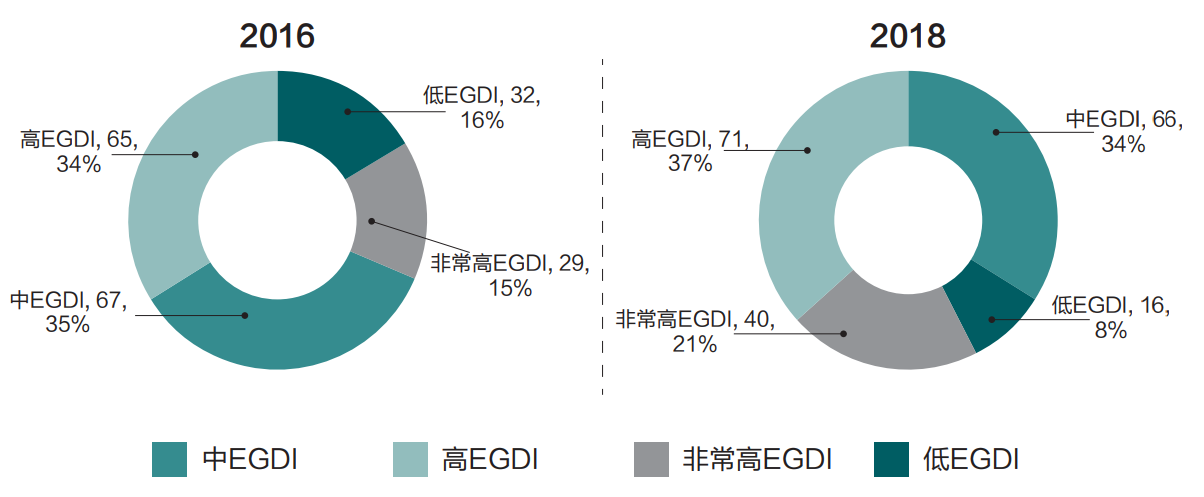
\includegraphics[width=0.9\linewidth]{figures/gov/1}
		\caption{2016年和2018年联合国电子政务发展指数(EGDI)分组国家数量对比
		{\tiny 《2018 联合国电子政务调查报告》数据显示,从地域分布上来看,非常高
		EGDI 国家中,欧洲国家占比较大,达到 67\%;在高 EGDI 组别中,亚洲和美洲
		国家最多,占比分别达到 33\%和 31\%;中 EGDI 组别中,非洲国家占比 50\%,且
		没有欧洲国家;低 EGDI 组别中,仅涉及两个大洲,非洲国家占比 87\%,亚洲国
		家占比 13\%}}
		\label{fig:1}
	\end{figure}
\end{frame}

\begin{frame}
	\frametitle{{中国电子政务发展现状}}
	\scriptsize
	\begin{minipage}[]{0.5\linewidth}
		\begin{enumerate}
			\item 2018 年中国电子政务发展指
			      数为 0.6811,排名 65 位,属于高 EGDI 国家,但与非常高 EGDI 国家仍有一定
			      差距。
			\item 截至 2019年6月,我国共有政府网站15143个,主要包括政府门户网站和部门
			      网站
			\item 我国32个省(区、市)和40多个国务院部门已全部开通网上政务服务平
			      台
			\item 截至2019年6月,我国在线政务服务用户规模
			      达到5.09亿,占总体网民的 59.6\%
		\end{enumerate}
	\end{minipage}%
	\begin{minipage}[]{0.05\linewidth}
		\quad
	\end{minipage}%
	\begin{minipage}[]{0.4\linewidth}
		\tiny
		\begin{tikzpicture}[scale=0.4]
			\pie[square, rotate=180, text=inside, color={blue!30, red!40, orange!70}]
			{42.1/微信支付宝城市服务, 23.6/政府微信公众号, 34.3/其他}
		\end{tikzpicture}

		\centering
		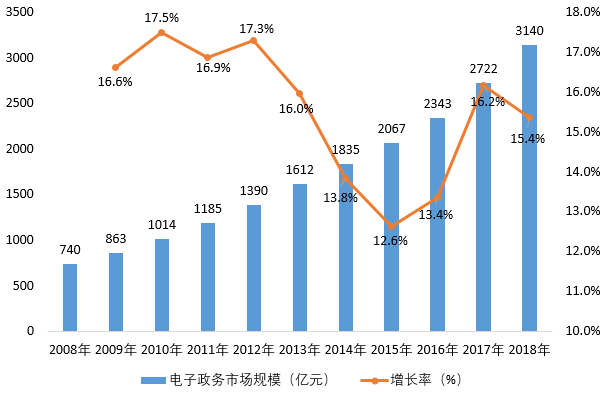
\includegraphics[width=0.9\linewidth]{figures/gov/2}
		\label{fig:2}
	\end{minipage}
\end{frame}

\begin{frame}
	\frametitle{{中国电子政务发展现状}}
	\begin{figure}
		\centering
		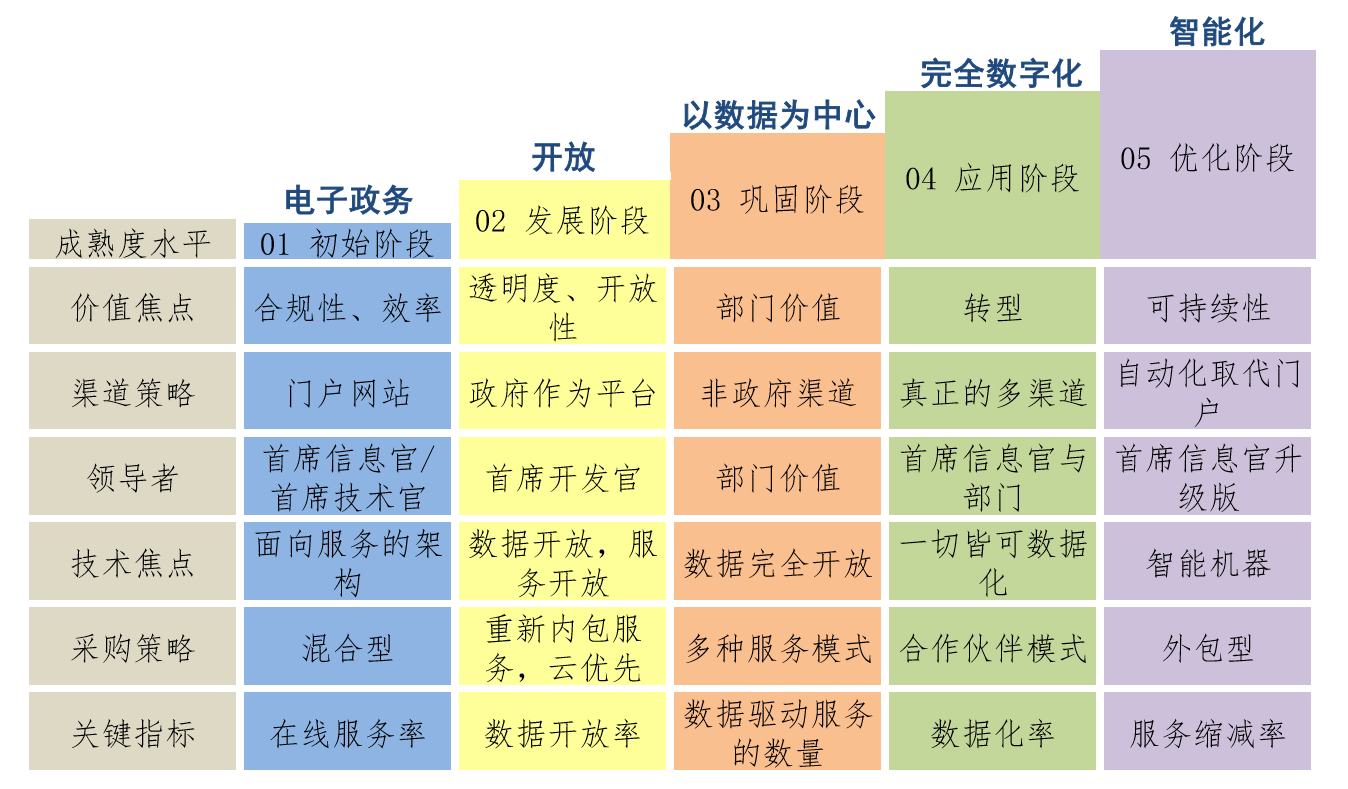
\includegraphics[width=0.75\linewidth]{figures/gov/3}
		\caption{Gartner 5 级电子政务成熟度模型}
		\label{fig:3}
	\end{figure}
	{\footnotesize 第三阶段-->第四阶段的转变期:具备规律性的跨组织数据流通,但缺乏标准导致电子政务数据的交互、协同、共享面临一定的困难。}
\end{frame}

\begin{frame}
	\frametitle{{电子政务实现阶段跨越的关键要素}}
	\begin{enumerate}
		\item 电子政务发展需均衡
		      \begin{enumerate}
			      \item 同级别不同行政区划的电子政务推进程度不同
			      \item 同地区不同部门间的电子政务推进程度不同
			      \item 现有的电子政务应用的广度与深度不足,无法对政府治理能力提升提供有
			            效支撑
		      \end{enumerate}
		\item 政务数据孤岛待打通

		      各部门之间的网络基础设施、业务系统、数据资源均处于割裂、碎片化状态,
		      没有形成标准统一的数据结构和数据接口,导致政务系统跨部门数据共享和业
		      务协同困难重重。
		\item 政务协同互信基础需加强

		      在现有的技术条件下,无法有效界定数据流通过程中的归属权、使用权
		      和管理权,若发生数据泄露事故将很难追溯数据泄露源头
		\item 城市数据监督需到位

		      在现有的政务信息化改革过程中,城市数据的治理与监督并未得到足够重
		      视,存在监管盲区和监管缺位。
	\end{enumerate}
\end{frame}

\subsection{区块链赋能政务信息化}
\begin{frame}
	\frametitle{习总书记发表重要讲话}
	\begin{enumerate}
		\item 2019 年
		      10 月 24 日,中共中央政治局就区块链技术发展现状和趋势进行第十八次集体学
		      习,习近平主持学习并发表重要讲话。其中针对区块链政务,习近平做出了细致
		      部署,“探索利用区块链数据共享模式,实现政务数据跨部门、跨区域共同维护
		      和利用,促进业务协同办理,深化‘最多跑一次’改革,为人民群众带来更好的政
		      务服务体验。
	\end{enumerate}
\end{frame}

\begin{frame}
	\frametitle{区块链赋能政务信息化}
	\begin{enumerate}
		\item 打通政务数据孤岛,深化“最多跑一次”改革
		\item 追溯数据流通过程,明晰数据权责界定
		\item 全生命周期管理,增强城市数据监督管控能力
		\item 构建分类共享体系,助力国家政务信息化工程建设
	\end{enumerate}
\end{frame}

\begin{frame}
	\frametitle{1、打通政务数据孤岛,深化“最多跑一次”改革}
	\begin{enumerate}
		\item 基于分布式记账技术、共识机制、非对称加密算法、智能合约等多种技术,现政务数据的授权共享、业务协同,夯实智慧政府基础
		\item 通过在各政府部门设立区块链节点,实现政务数据共享过程的数据确权、控制信息计算、个性化安全加密等
		\item 利用区块链的“去信任化”特性,打通政务数据孤岛,为原有部门条块化的数据授权共享与业务协同提供技术基础
		\item 结合安全多方计算等技术,各政府部门可以在无需对外提供原始数据的前提下,实现对与其数据有关的函数计算,解决了一组互不信任的参与方之间保护隐私的协同计算问题
	\end{enumerate}
\end{frame}

\begin{frame}
	\frametitle{2、追溯数据流通过程,明晰数据权责界定}
	\begin{enumerate}
		\item 去信任化是区块链技术与生俱来的特性之一,将区块链与政务信息化深度融合,能够建立各部门间的信任和共识,夯实各协作部门的信任基础,实现在确保数据安全的同时促进各部门数据的授权共享与业务协同
		\item 区块链技术能够对数据流通过程可信追溯,为有效解决政务数据使用过程中归属权、管理权和使用权的界定难题提供技术支撑。在区块链网络中,结合公私钥体系,政务数据一经产生就确定了归属权与管理权,为后续的授权使用明晰了权责,进一步结合智能合约技术,能够明晰数据共享与业务协同过程中的
		      使用权
		\item 在政务数据授权共享、业务协同的同时,能够将所有的数据流转使用记录留存于链上,基于区块链所具有的不可篡改、可溯源的特性,可为后续数据泄露等事故提供有迹可循的、清晰的溯源依据,为建立可监管、可追溯的政务数据共享授权机制扫清道路
	\end{enumerate}
\end{frame}

\begin{frame}
	\frametitle{3、全生命周期管理,增强城市数据监督管控能力}
	\begin{enumerate}
		\item 区块链基于点对点的分布式账本技术、哈希指针与时间戳技术,确保了数据
		      一旦上链无法篡改,且具有可溯源的特性。
		\item 在城市治理中,城市数据的应用具有十分重要的作用。区块链具有不可篡改
		      性,结合物联网技术,能够实现城市政务数据的全流程存证,扫清原本因技术局
		      限无法覆盖的监督盲区,补足监管的缺位,增强城市数据监督管控能力,为后期
		      的核验、举证等提供便利,提升政府公信力。比如在政府重大投资项目上实行建
		      设主体的全流程数据上链,利用区块链不可篡改性和可追溯性,将对其产生较大
		      约束力。
		\item 此外,通过将相关监管机构、企业等纳入区块链生态,通过数据上链促使监
		      管机构实现更全面的监管,营造良好的营商环境,并为实现基于数据的科学决策
		      提供坚实支撑。比如在财务税务上,通过将税务机关、开票企业、纳税人和报销企业纳入区块链网络,能够大幅缩减报销流程,解决发票报销中的一票多报等问
		      题,还能够有效防止偷税漏税,降低税局稽查成本,提升监管机构的监管效力。
	\end{enumerate}
\end{frame}

\begin{frame}
	\frametitle{4、全生命周期管理,增强城市数据监督管控能力}
	\begin{enumerate}
		\item 按照《政务信息资源共享管理暂行办法》,政务数据分为无条件共享、
		      有条件共享、不予共享等三种类型
		\item 依托公私钥保密体系和智能合约技术,区块链能够为构建政务数据分类共享
		      体系赋能。通过完善政务数据信息资源目录体系和分类共享体系,结合区块链的
		      公私钥与智能合约,能够实现不同共享类型数据的依权限分类共享,提高安全保
		      障能力
	\end{enumerate}
\end{frame}

\subsection{区块链政务应用落地难点}
\begin{frame}
	\frametitle{区块链政务应用落地现状}
	\begin{figure}
		\centering
		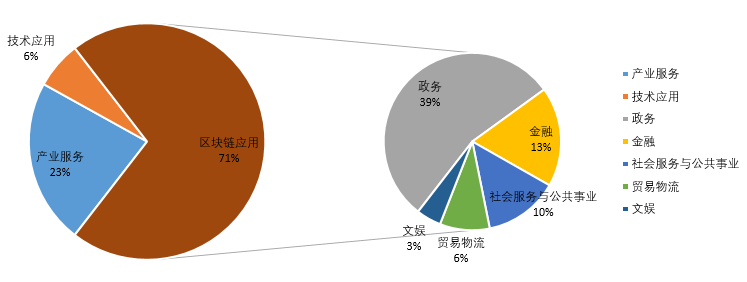
\includegraphics[width=0.9\linewidth]{figures/gov/4}
		\caption{2019 年政府采购区块链项目类别}
		\label{fig:4}
	\end{figure}
	{\footnotesize 区块链政务
	应用涉及到数字身份、电子存证、电子票据、产权登记、工商注册、数据共享、
	涉公监管、行政审批等诸多场景。尽管已有一定数量的区块链政务应用落地,但
	总体来说仍属于小范围尝试,这些先行者在探索的路上也面临一些难题。}
\end{frame}

\begin{frame}
	\frametitle{区块链政务应用落地难点}
	\begin{enumerate}
		\item 标准规范未统一,相关制度待完善
		\item 业务梳理难度大,系统安全需谨慎
		\item 系统潜力未深挖,重复建设难避免
	\end{enumerate}
\end{frame}

\subsection{区块链政务发展趋势与展望}
\begin{frame}
	\frametitle{区块链政务发展趋势与展望}
	\begin{enumerate}
		\item 坚持以人为本,优化政务服务
		\item 强化顶层设计,产学研用协同
		\item 完善相关制度,营造良好环境
		\item 释放数据红利,建设智慧政府
	\end{enumerate}
\end{frame}

\subsection{区块链政务应用探索与实践}
\begin{frame}
	\frametitle{区块链服务网络(BSN)——BSN 政务专网}
	\begin{figure}
		\centering
		
\includegraphics[width=0.7\linewidth]{figures/gov/6}
		\caption{BSN 政务专网结构}
		\label{fig:6}
	\end{figure}

	区块链服务网络(BSN)由国家信息中心顶层设计,中国移动通信集团公司、
	中国银联股份有限公司、北京红枣科技有限公司等单位共同建设的首个国家级联
	盟链应用底层公共基础设施,致力于打造跨公网、跨地域、跨机构的区块链服务
	网络。
\end{frame}

\begin{frame}[allowframebreaks]
	\frametitle{深圳市区块链电子发票}
	\begin{figure}
		\centering
		
\includegraphics[width=0.6\linewidth]{figures/gov/8}
		\label{fig:8}
	\end{figure}
	{\footnotesize 	\begin{enumerate}
		\item 税务机关将开票规则部署上链,包括开票限制性条件等,税务机关在链
		      上实时核准和管控开票
		\item 开票企业申领发票,将订单信息和链上身份标识上链
		\item 纳税人认领发票,并在链上更新纳税人身份标识
		\item 收票企业验收发票,锁定链上发票状态,审核入账,更新链上发票状态,
		      最后支付报销款
	\end{enumerate}}
	{\footnotesize 	腾讯区块链电子发票底层采用区块链技术,借助分布式记账、多方共识和非堆成加密等技术,实现发票开具与线上支付相结合的效果,打通了发票申领、开
	票、报销和报税的整体流程}

	解决痛点:
	\begin{enumerate}
		\item 打通信息孤岛。通过区块链连接了每一个发票干系人,发票信息实时上链,
		      实现发票状态的全流程可查可追溯
		\item 简化报销流程。发票干系人通过链上协作,实现无纸化报销,并且链上报销
		      无需繁琐的手续,简化了报销流程
		\item 解决“一票多报,虚抵虚报”问题。利用区块链技术,可以确保发票的唯一性
		      和信息记录的不可篡改性
		\item 加强政府监管力度。由于发票信息上链,公开透明、无法篡改且可溯源,为
		      税局提供了更好的实时性全流程监管手段
	\end{enumerate}
\end{frame}

\begin{frame}[allowframebreaks]
	\frametitle{红普可信多方计算和管理系统}
	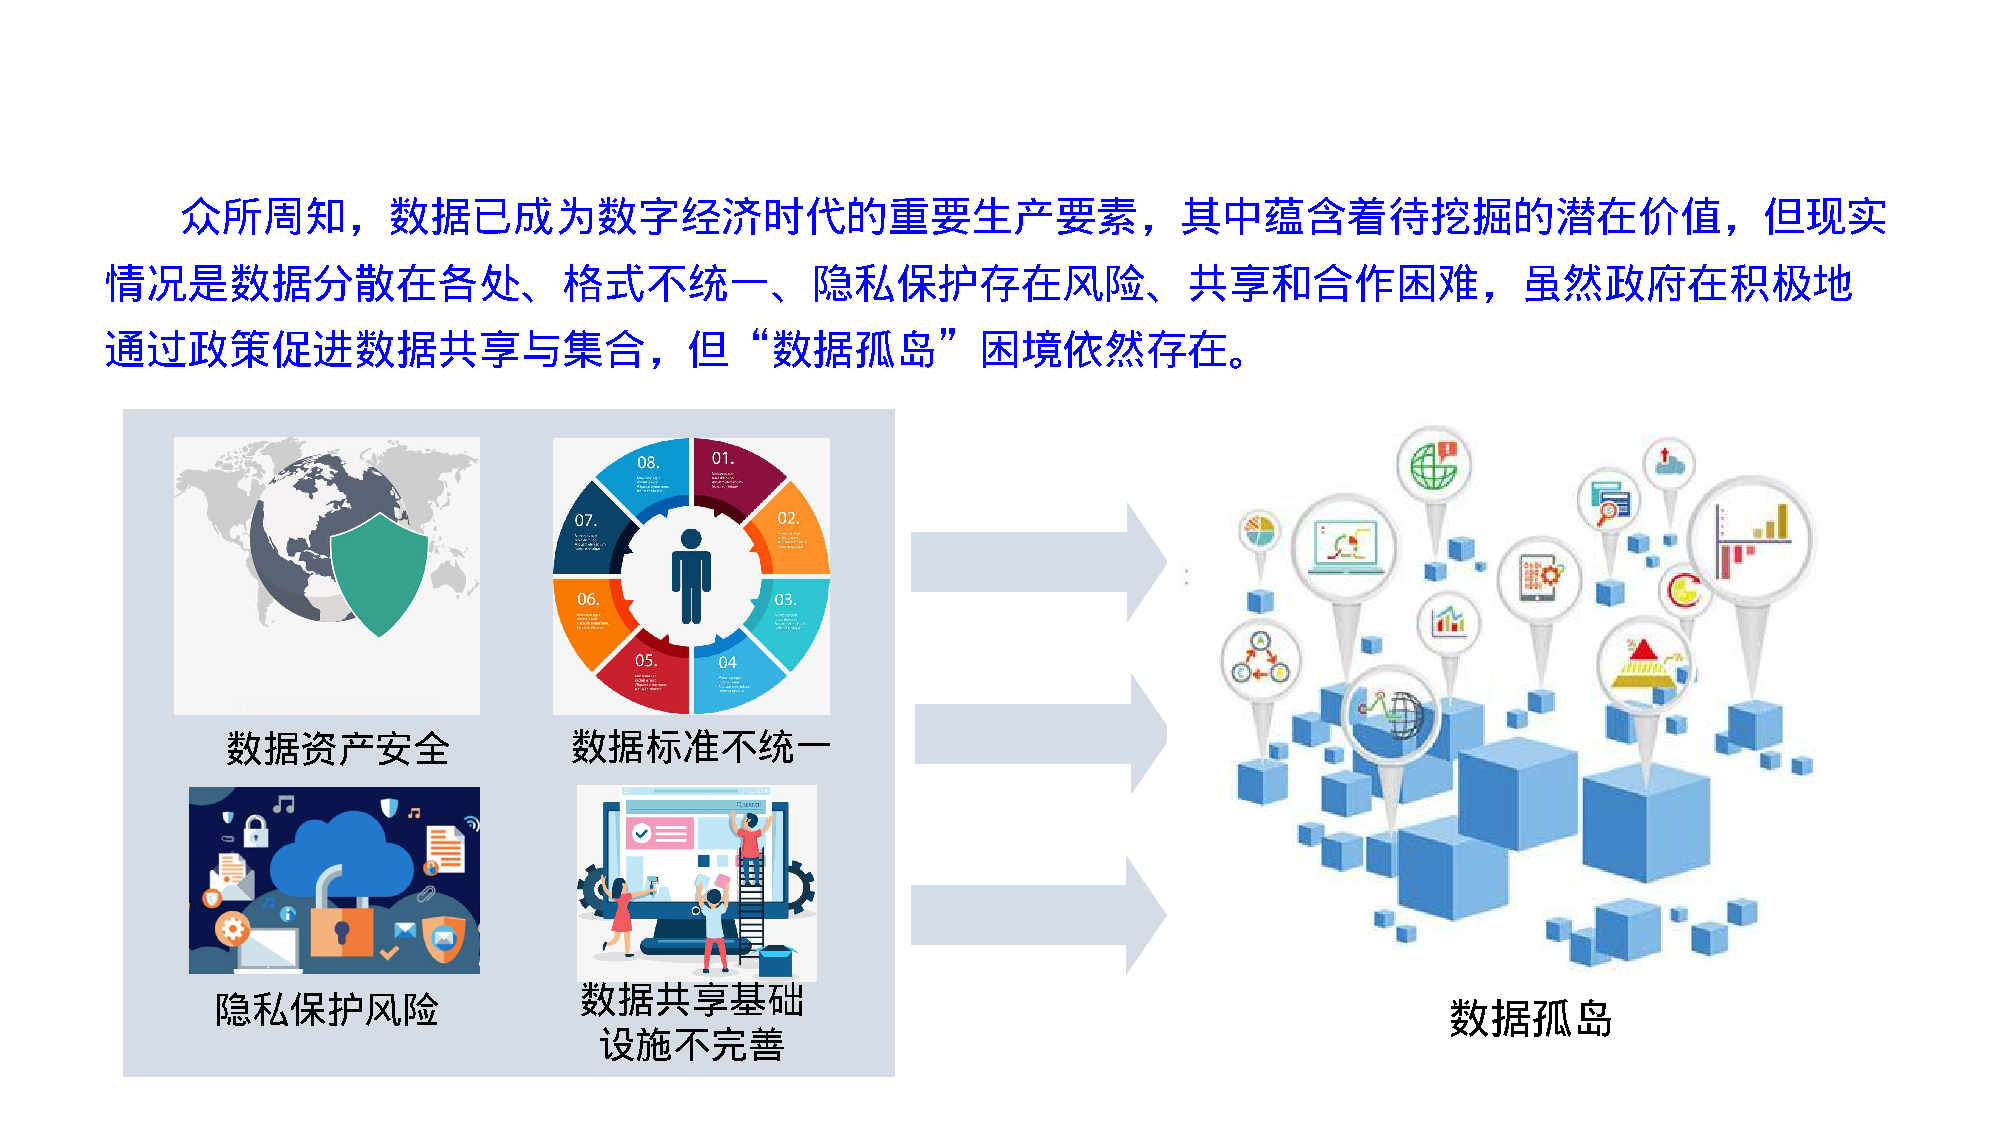
\includegraphics[page=1,width=\textwidth]{figures/gov/hmb.pdf}
	
	\includegraphics[page=2,width=\textwidth]{figures/gov/hmb.pdf}
\end{frame}



\section{区块链数字身份:数字经济时代基础设施}

\begin{frame}
	\frametitle{}
{\Large 	区块链数字身份:数字经济时代基础设施}
\end{frame}

\subsection{传统数字身份的运行逻辑}
\begin{frame}
	\frametitle{数字身份的含义}
	\begin{enumerate}
		\item
		      身份载体的演变:纸质->电子信息,衍生出数字身份
		\item  身份内涵的拓展:人->人、物
		\item 数字身份的四个环节:注册、签发、验证和管理
		      \begin{enumerate}
			      \item 注册:身份所有者注册
			      \item 签发:身份提供方签发身份标识
			      \item 验证:身份提供方或依赖方验证
			      \item 管理:身份所有者、身份提供者参与管理,身份的储存、更新、撤销、授权
			            等
		      \end{enumerate}
	\end{enumerate}
\end{frame}

\begin{frame}
	\frametitle{数字身份认证与管理}
	\begin{enumerate}
		\item 身份认证的密码学算法
		\item 身份认证的实现
		      \begin{enumerate}
			      \item 口令
			      \item 智能卡
			      \item 生物特征识别
			      \item 数字签名
			      \item 数字证书
		      \end{enumerate}
		\item 传统身份认证管理系统:PKI(公钥基础设施)
	\end{enumerate}
\end{frame}

\subsection{数字身份市场发展现状与趋势}
\begin{frame}
	\frametitle{数字身份市场现状}
	\begin{figure}
		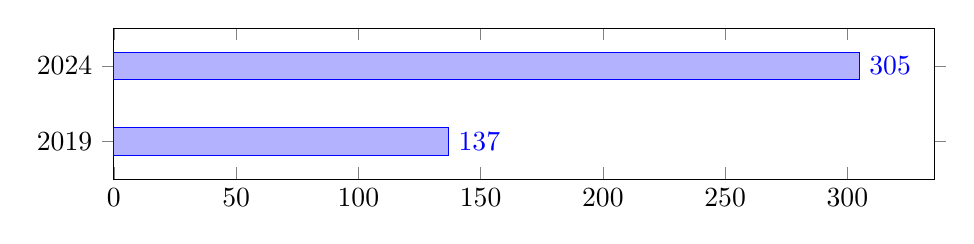
\begin{tikzpicture}
			\begin{axis}[
					xbar, xmin=0,
					width=12cm, height=3.5cm, enlarge y limits=0.5,
					symbolic y coords={2019,2024},
					ytick=data,
					nodes near coords, nodes near coords align={horizontal},
				]
				\addplot coordinates {(137,2019) (305,2024)};
			\end{axis}
		\end{tikzpicture}
		\caption{全球数字身份市场规模(亿美元)与增长率\footnote{MarketsandMarkets}}
	\end{figure}
	预测期内,亚太地区将以最高复合增长率增长。当下,中国、日本和新加坡
	等国家已经开始在各个垂直领域实施数字身份解决方案,包括银行、金融服务和
	保险(BFSI)、医疗、政府和国防垂直领域。
\end{frame}

\begin{frame}[allowframebreaks]
	\frametitle{现有数字身份的痛点}
	\begin{enumerate}
		\item 身份数据分散和重复认证
		\begin{example}
			对金融 KYC 来说,
			同一个公民去不同的银行需要做不同的 KYC。 这些身份数据中很多相互重叠
			\begin{enumerate}
				\item 一方面造成了资源存储的浪费
				\item 另一方面也给用户使用身份带来了不便与低效
				\item 往往需要重复注册和认证
				\item 不同身份系统中的用户身份数据由各系统单独存储,
				无法共享和流通,也无法综合利用
			\end{enumerate}
		\end{example}
	
		现有解决方案:OAuth 2.0
		\item 中心化认证效率和容错性低
		\begin{example}
			现有PKI体系CA机构为树型结构
			\begin{enumerate}
				\item 一方面,这种中心结构可能存在性能问题,其涉及证书的所有
				操作,任务繁重,可能成为性能短板拖累效率。
				\item 另一方面则是安全问题,这种单中心的结构容易使其成为攻击的目标,
				一旦中心失效,则左右与之关联的下级 CA 均会收到牵连
			\end{enumerate}
		\end{example}
		\item 身份数据隐私与安全
		
		{\scriptsize 现有数字身份信息散落在各个身份认证者手中,服务方可能在未获用户授权的情况下对这些数据进行处置,几乎毫
无顾忌地收集、存储、传输、买卖用户,这实际上是对于用户隐私信息的严重侵
		犯。}
	
		2018 年 5 月,欧盟正式推出通用数据保护条例(GDPR),其目的在于遏制
		个人信息被滥用,保护个人隐私。
		
		\item 传统身份证明无法覆盖所有人
		
		\begin{example}
			球大约有 11 亿人没有
			官方身份证明,包括大量的难民、儿童和一部分妇女,他们可能无法获得应有的
			权利,比如教育、医疗、保险、金融等。 他们虽然可以拥有一些非官方提供的身
			份,但却缺乏足够的信任,支撑他们获得应有的权利。
		\end{example}
	\end{enumerate}
\end{frame}

\begin{frame}
	\frametitle{数字身份的演变与主权身份的崛起}
	基于对统一认证、数据隐私等等的需求,数字身份也出现了多种的转变与探
	讨,逐渐向着自我主权身份的要求转变
	\begin{enumerate}
		\item 集中式身份:目前最主流身份认证方式
		\item 联盟身份:最终形成了身份信息垄断的格局
		\item 以用户为中心的身份:存在隐私泄露风险,用户并没有取得身份的自主权
		\item 自我主权身份:基于区块链实现分散信任的环境,提供可信身份
	\end{enumerate}
\end{frame}

\subsection{区块链与数字身份的结合形式}

\subsubsection{区块链实现数字身份的可信互认}
\begin{frame}[allowframebreaks]
	\frametitle{1、区块链实现数字身份的可信互认}
	{\scriptsize 当前在自我主权身份发展早期的阶段,前三个阶段的数字身份形式仍然是最
	主流的。本节主要探讨如何运用区块链技术改善传统数字身份认证方式,提高安
	全性和数据共享。}
\begin{enumerate}
	\item 分布式身份认证:针对 CA 的中心化签发所引发如中心失效、网络安全等问题
	\begin{enumerate}
		\item 区块链的分布式的数字证书签发,集中式 CA 认证中心签发数字证书-->区块链的分布式账本实现
		\item 所有证书持有者共同维护。 基于区块链的 PKI 可以实现传
		统 PKI 系统的证书申请、签发、验证和管理
		\begin{enumerate}
			\item 证书签发:用户自己生成公私钥对,私钥自己保存,并将公钥和用于
			验证个人身份信息的数据发动给验证节点进行证书的申请。
			\item 证书签发: 会根据新用户提交的信息验证其身份的真实性;验证通过
			后生成数字证书并上链。
			\item 证书撤销:证书用户提出证书撤销请求,其中包括用户的证书以及可
			以证实用户身份的信息; 验证节点根据用户提交的信息验证用户身份,审核证书
			撤销请求通过后, 将未纳入区块的合法证书信息以及证书状态上链。
			\item 证书更新:用户需要产生一份新的数字证书,与原有证书有相同的 DN
			(Distinguished Name)项。证书用户向区块链网络发起证书更新请求,提交待更
			新的证书,新产生的证书以及证实身份的信息。其后再由验证节点进行验证上链
		\end{enumerate}
	\end{enumerate}
\end{enumerate}
\end{frame}

\begin{frame}
	\frametitle{2、跨机构安全身份授权}
	{\scriptsize 目前数字身份数据分散, 难以共享, 传统的身份授权方式不够安全。 在统一
		身份标识无法快速实现和成熟的背景下,可以利用区块链的分布式账本让身份共
		享和授权更加安全}
	\begin{minipage}[t]{0.5\linewidth}
	\begin{figure}
	\centering
	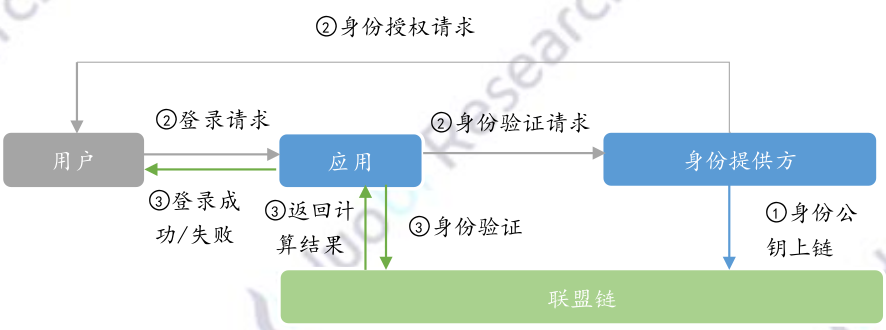
\includegraphics[width=\linewidth]{figures/eid/1}
	\caption{跨机构区块链身份授权流程}
\end{figure}
\end{minipage}%
\begin{minipage}[t]{0.5\linewidth}
{\scriptsize 	\begin{enumerate}
		\item 拥有用户数据的服务商将用户信息加密生成私钥和公钥,
		\item 
		其中公钥生成该
		运营商的数字签名,将公钥和数字签名上链,私钥则保存在用户本地,如 SIM 卡。
		\item  用户登录联盟链中某一应用(依赖方)时,该应用会向有用户身份信息的
		服务商(身份提供方)发起请求,接收到请求后,服务商向用户发送授权申请,
		等待用户同意。
		\item  应用获得用户授权后,在链上对用户身份进行匹配,匹配成功后即说明对用户身份认可,可以登录。
\end{enumerate}}
\end{minipage}%
\end{frame}

\begin{frame}[allowframebreaks]
	\frametitle{3、区块链数字身份提供可信基础设施}
\begin{enumerate}
	\item 区块链技术可以和生物识别技术相结合,创建真实唯一,难以伪造的
	数字身份。
	\begin{example}
		如指纹、面部、虹
		膜等,提取其二进制特征向量, 经过 Hash 处理后以数字摘要的形式存储在区块
		链上,形成不可篡改的数字身份,代替传统所需的 ID 号
	\end{example}
	\item 可以利用区块链形成用户不可篡改的行为记录,与其身份绑定,增强
	其身份特性和可信行为特性
	
	{\tiny 2017 年世界上仍有 17 亿人没有银行账户。这是一个十分惊人的数字,
	这意味着世界上有 17 亿人无法利用银行进行基本的储蓄、汇款等业务。而更重
	要的是,银行绝大部分现有金融服务又依赖于客户的 KYC 情况、过往金融记录
	等银行数据,而很难将金融服务延伸给这些真正需要融资的贫困人群等。通过区
	块链数字身份,可以对很多以往无法统计的金融行为进行记录,由于信息的不可
	篡改性,用户的金融信用会加强,更有助于其获得金融机构的认可,能够实现应
	用的金融权利}
\end{enumerate}
\end{frame}

\subsection{区块链实现自我主权身份与数据管理}
\begin{frame}[allowframebreaks]
	\frametitle{实现用户数据自治:分布式身份标识}
	基于区块链的自我主权身份的核心思想是创造一个全局唯一的身份标识
	DID(分布式身份标识),具有高可用性、可解析性和加密可验证性。

	\begin{minipage}[t]{0.5\linewidth}
	\begin{figure}
		\centering
		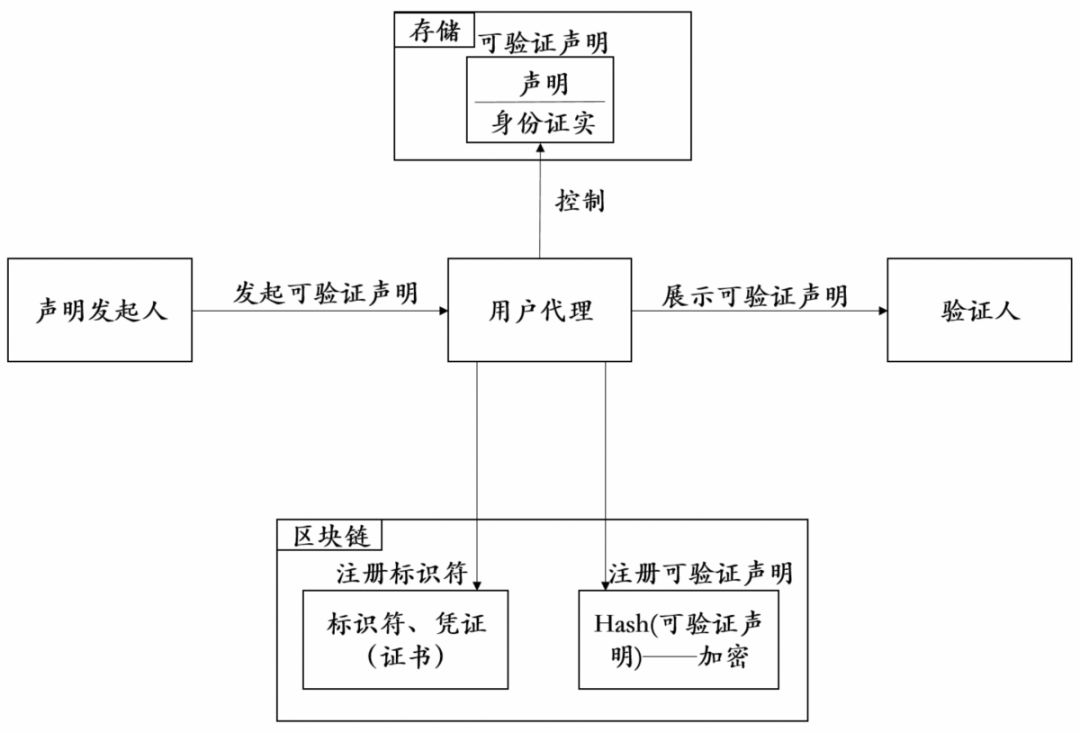
\includegraphics[width=\linewidth]{figures/eid/2}
		\caption{DID 系统运行流程}
	\end{figure}
\end{minipage}%
\begin{minipage}[t]{0.5\linewidth}
{\footnotesize 	\begin{enumerate}
	\item DID 标识符:是全局唯一的身份标识,类似一个人的身份证、账号等。
	\item DID 文档:描述如何使用该 DID 的简单文档。
	\item 可验证声明(VC): DID 文档本身无法和用户的真实身份信息相关联,
	需要 VC 来实现,是整个系统的价值所在。
\end{enumerate}}
\end{minipage}%
\end{frame}

\begin{frame}[allowframebreaks]
	\frametitle{数据隐私保护的解决思路}
\begin{enumerate}
	\item 零知识证明(Zero-Knowledge Proof):{\tiny 指的是可以在不泄露任何其他
		信息的前提下证明一个命题的正确性。这里的“零知识”并不是什么都不知道,而
		是什么都不泄露。身份认证是零知识证明的典型应用,例如匿名认证(通过认证
		并获得相应的权限,却不泄露身份),保护用户的隐私。零知识证明可以结合可
		验证声明为身份依赖者提供身份验证,比如证明你已经成年,却不会暴露你的真
		实年龄。对于身份依赖方来说,其实就是匿名形式的认证。}
	\item 分布式密钥管理:{\tiny 指的是将密钥进行分片,多个密钥碎片分布式存储,
		必须要大于一定比例的密钥碎片才能够合成完整的密钥。密钥碎片可以由区块链
		网络节点进行管理,相比如公钥直接上链具有更强的安全性和隐私性,加强了数
		字证书的不可篡改性。}
	\item 可信执行环境(TEE,Trusted Execution Environment):{\tiny 基于芯片硬
		件形成的可信环境,能够对敏感数据进行有效保护。TEE 隔离于 REE(移动设备
		运行 OS 的环境)、只能通过特定的入口与 TEE 通信;TEE 可以访问 REE 的内
		存、 REE 无法访问受硬件保护的 TEE 内存; TEE 还可抵御某些基于硬件的攻击。
		因此 TEE 常用于数据内容版权保护、金融支付、身份认证等场景。在身份认证中,TEE 可用于保护本地的用户隐私数据以及用户的密钥。}
	\item 安全多方计算(Secure Multi-Party Computation):{\tiny 该方案主要针对无
	可信第三方的情况下,如何安全地计算一个约定函数的问题。参与计算的各方可
	以在不泄露自己的数据的前提下,共同完成某个计算过程,并且最终的计算结果
	还能证明是正确的。安全多方计算可以解决大数据时代,有价值的数据或是隐私
	数据难以分享的痛点,例如身份数据,金融数据等。在安全多方计算的协助下,
	多个数据持有方才能更放心的开展合作,在不损害自身利益的情况下,创造更大
	的价值。}
\end{enumerate}
\end{frame}

\subsection{应用案例}

\begin{frame}
	\frametitle{实现用户数据自治:分布式身份标识}
	eID 数字身份链是以国家 863 重大专项公民数字身份为基础的国家数字基础
	设施。通过对接联合国家各部委和有关部门,建立链接个人各维度数据的个人隐
	私保护体系和数据流转平台。
	
	\begin{minipage}[t]{0.5\linewidth}
		\begin{figure}
			\centering
			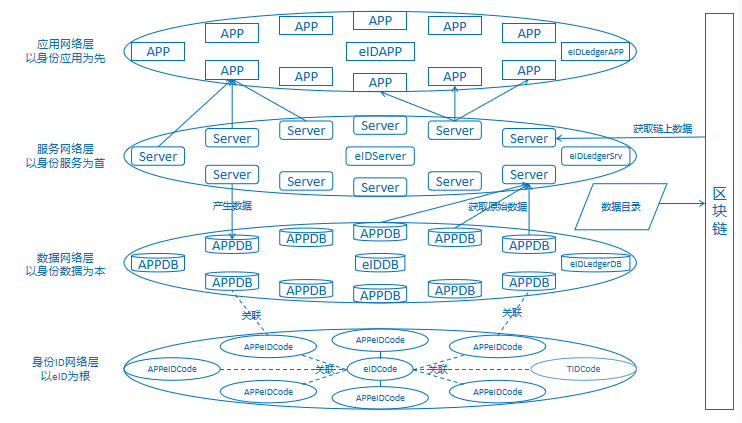
\includegraphics[width=\linewidth]{figures/eid/3}
			\caption{eID 数字身份链技术框架图}
		\end{figure}
	\end{minipage}%
	\begin{minipage}[t]{0.5\linewidth}
		\begin{figure}
	\centering
	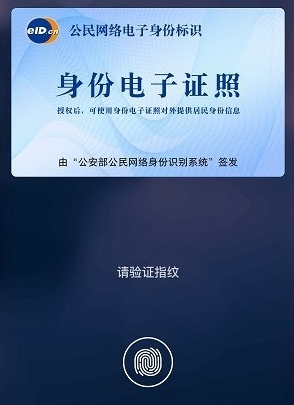
\includegraphics[height=0.5\linewidth]{figures/eid/4}
	\caption{案例:eID 数字身份的区块链电子证照}
\end{figure}
	\end{minipage}
\end{frame}

\subsection{区块链数字身份的难点}
\begin{frame}
	\frametitle{1、区块链与隐私保护技术的低效问题}
	\begin{enumerate}
		\item 共识算法和区块链查询的效率比较低
		\item 基于零知识证明的隐私保护技术依赖双方的多次交互来进行,效率底下。未来如果要使用安全多方计算,对网络资源的依赖会更加严重
		\item 分布式身份受到网络和共识的影响会限制其发展
	\end{enumerate}
\end{frame}

\begin{frame}
	\frametitle{2、用户数据隐私与企业数据变现的现实冲突}
	\begin{enumerate}
		\item 身份数据分散和重复认证
		\item 中心化认证效率和容错性低
		\item 身份数据隐私与安全
		\item 传统身份证明无法覆盖所有人
	\end{enumerate}
\end{frame}

\begin{frame}
	\frametitle{3、私钥管理和身份标识符的使用门槛较高}
	\begin{enumerate}
		\item 身份数据分散和重复认证
		\item 中心化认证效率和容错性低
		\item 身份数据隐私与安全
		\item 传统身份证明无法覆盖所有人
	\end{enumerate}
\end{frame}

%
%\section{区块链构建智慧城市运转新内核}
%
%\section{区块链下的“普惠”供应链金融}
%
%\section{区块链开启医疗健康新篇章}
\end{document}